%
%  This is an example LaTeX file. The percent sign is used to mark the
% start of a comment.
%
%  - Michael Weeks, January, 2003
%
\documentclass[conference]{IEEEconf}
\usepackage[dvips]{graphics}
\usepackage{tikz}
\usepackage{dtklogos}
\usepackage[utf8]{inputenc}
\usetikzlibrary{mindmap}
\usepackage[hidelinks,pdfencoding=auto]{hyperref}
% Information boxes
\newcommand*{\info}[4][16.3]{%
  \node [ annotation, #3, scale=0.65, text width = #1em,
          inner sep = 2mm ] at (#2) {%
  \list{$\bullet$}{\topsep=0pt\itemsep=0pt\parsep=0pt
    \parskip=0pt\labelwidth=8pt\leftmargin=8pt
    \itemindent=0pt\labelsep=2pt}%
    #4
  \endlist
  };
}

\IEEEoverridecommandlockouts % Don't forget this command!

\begin{document}
  \title{Data Driven Approach For Transfer Data  From ANT+ Sensors}

  \author{{Petr Je\v{z}ek$^{1}$, Roman Mou\v{c}ek$^{1}$}
\thanks{$^{1}$Department of Computer Science and Engineering
New Technologies for the Information Society
Faculty of Applied Sciences
University of West Bohemia
Plzen, Czech Republic
        {\tt\small {jezekp, moucek}@kiv.zcu.cz}}%
\thanks{*Acknowledgements will be added}% <-this % stops a space
}
\maketitle


\begin{abstract}
This is the abstract. You can use this file to start your own LaTeX file,
and just delete the stuff you do not need. \LaTeX  is a lot like working
with HTML: you can specify where text effects begin, and where they end.
\end{abstract}

\section{Introduction}\label{sec:intro}
Managing diseases and health issues is worldwide still more expensive especially with aging population. For instance there are around 23 million people affected with heart failure \cite{bui2011epidemiology}. These people have been treated in hospitals for a long time. Nowadays, the situation is changing because relatively cheap solutions for a home treatment is coming to the market \cite{4761985, 5333913}. These solutions enable to make a particular shift of patients from hospitals to their homes. It brings advantages in better comfort for patients and cheapens treatment itself. These solutions usually use a set of sensors for monitoring of a health level. Wearable sensors are usually powered from batteries. They have to operate for a long time period without possibility to change batteries frequently. As a solution new protocols with the objective of low energy consumption as ZigBee \cite{Farahani:2008:ZWN:1457417}, Bluetooth Low Energy \cite{heydon2012bluetooth} or ANT \cite{zaloker2014ant} has been defined.  Data from these sensors are transfered to remote servers where they are processed and results are visualized to the user. Sensors usually measure a large collection of body parameters. Integration of these sensors creates a Body Area Networks (BAN). When the number of sensors connected to BAN is increasing a management and a long term storage and sustainability of data is a major requirement in future applications.

While low energy consumption standards for data transfer exist they are still too fragmented to enable an easy manipulation with obtained data. As a solution this paper presents an approach of using a unified HDF5 format for encapsulating ANT+ sensor data and its transfer to a remote storage. 

The paper is organized as follows. Section \ref{sec:state-of-the-art} describes current approaches in the domain then Section \ref{sec:ant-plus-profiles} describes existing ANT+ profiles and selects most suitable profiles for eHealth domain. Section \ref{sec:framework} describes proposed framework that facilitates the conversion of sensors data to an output HDF5 format. Then Section \ref{sec:use-case} demonstrates the usage of proposed transformation. Last Section \ref{sec:future-work} summarizes the current work and provide an outlook to the future.

\section{State of The Art}\label{sec:state-of-the-art}

An approach presented in \cite{mehmood2014ontology} defines a three layers ontology describing data from different sensors. This ontology can facilitates programmer development of tools for processing sensors data. A Sensor-Cloud infrastructure \cite{5635688} represents physical sensors as virtual sensors stored in a Cloud infrastructure. The Cloud manages sensors capability. So called Semantic Sensor Web \cite{4557983} is based on an annotation of sensors data by means of Semantic Web. Such annotated data can be distributed via the Internet.


\section{ANT+ Profiles Discussion}\label{sec:ant-plus-profiles}
ANT+ protocol is popular because of its low energy consumption and because it provide good means to describe body parameters or fitness level. The main benefit are ``device profiles`` to define how to send data over the network in a consistent way \cite{innovations2013ant}. When the data transfer profiles are defined they facilitates development of sensors. 
ANT+ profiles supports a large scale of activities such as Cycling, Walking or devices for measurement of Heart Rate, Blood pressure, Weight, Muscle Oxygen Monitor etc. If we browse individual profiles detailed we can observe attributes that are common for all profiles including e.g.: device name, status, manufacturer, signal strength or battery status. Then, there are other attributes varying for individual profiles. 

According to individual attributes of profiles we can define common attributes as metadata of sensors and individual profile attributes as raw data. 

\section{Proposed Framework}\label{sec:framework}

Although several APIs for processing data coming from ANT+ devices exist their transfer to remote databases is not satisfactorily solved. When data have to be transfered and stored a unified data format has to be defined.

As a solution we are here presenting a Framework that expresses data in 

\begin{figure*}[ht]
\centering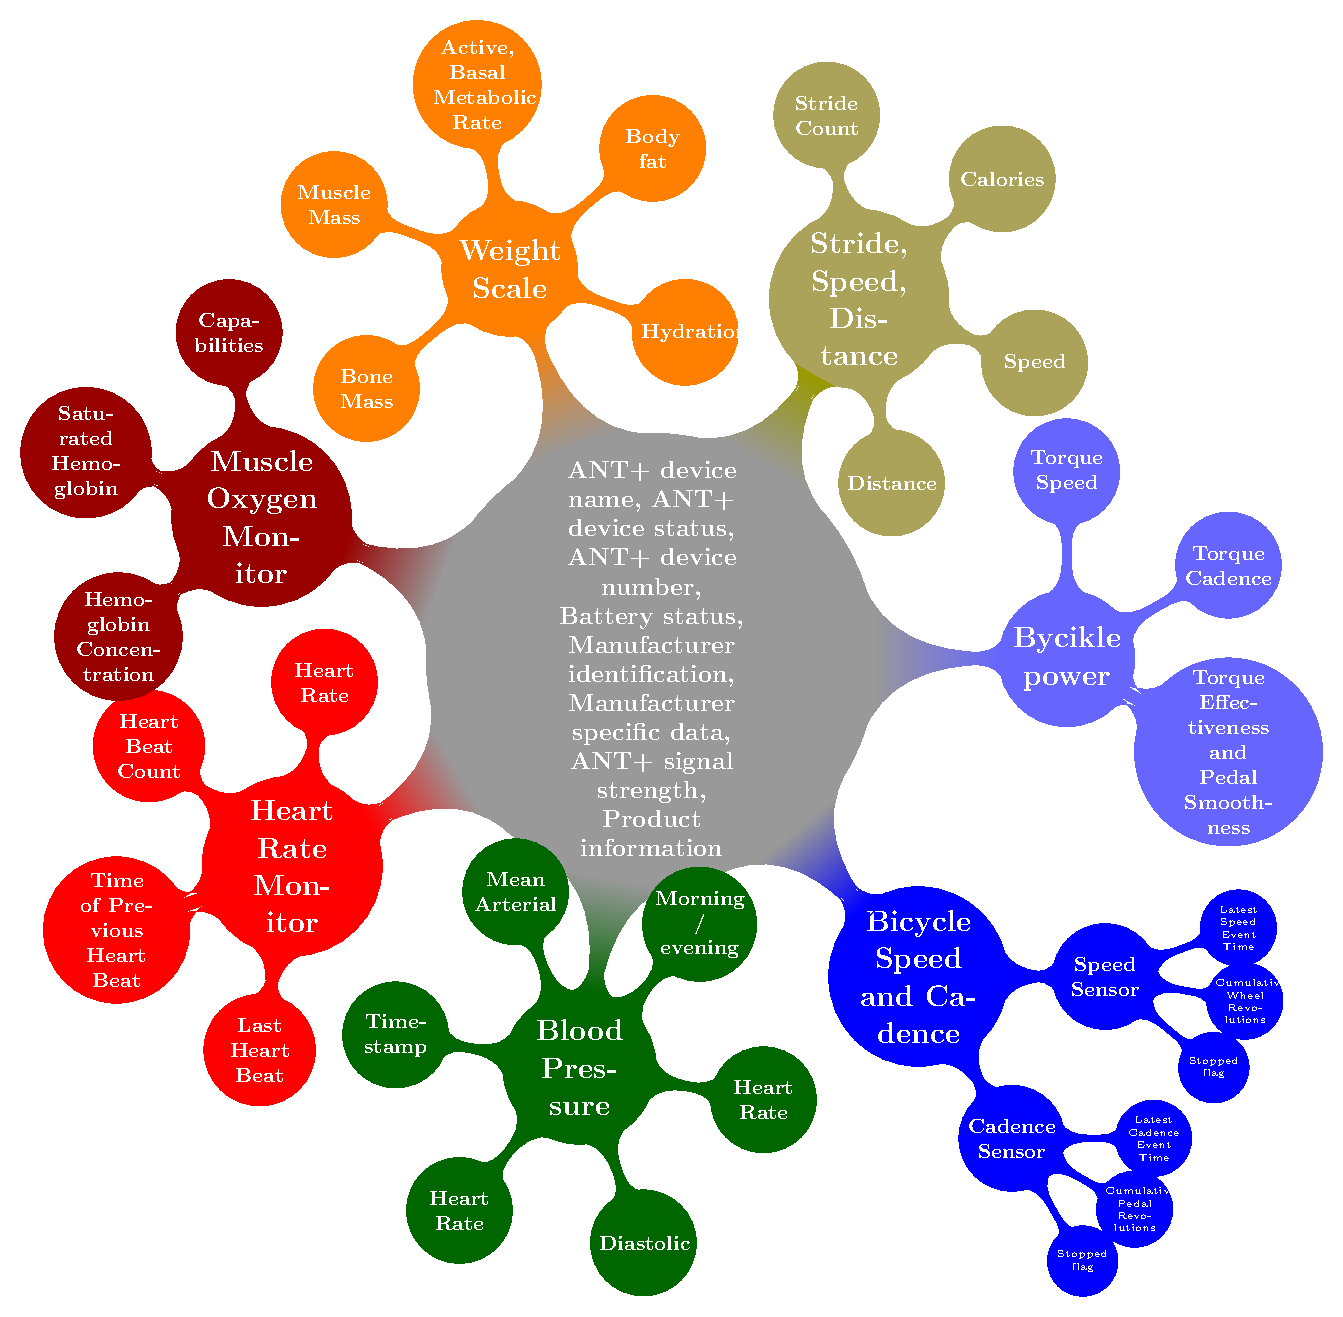
\includegraphics[width=12cm, height=10cm]{AntPlusProfiles}
\caption{\label{AntPlus}ANT+ Profiles Network}
\end{figure*}

\subsection{Format Discussion}
\subsection{Proposed Mapping}
\subsection{Implementation}

\section{Use Case}\label{sec:use-case}

\section{Conclusions and Future Work}\label{sec:future-work}





% Now here is the reference section.

\bibliographystyle{IEEEtran}
% argument is your BibTeX string definitions and bibliography database(s)
\bibliography{EMBC-2016}
\end{document}